\begin{center}
  \section*{Vision of \\ St. Thomas' College of Engineering \& Technology}
\end{center}

\justify
To evolve as an industry oriented, research based Institution with ethical values for creative solutions in various engineering domains, with an ultimate objective of meeting technological challenges faced by the Nation and the Society.

\begin{center}
  \section*{Mission of \\ St. Thomas' College of Engineering \& Technology}
\end{center}

\begin{itemize}
  \item \textbf{M1:} To enhance the quality of engineering education and delivery through accessible, comprehensive and research oriented teaching-learning-assessment processes in the state-of-art environment.
  \item \textbf{M2:} To create opportunities for students and faculty members to acquire professional knowledge with multidisciplinary approach and develop managerial, entrepreneurial and social attitudes with highly ethical and moral values.
  \item \textbf{M3:} To satisfy the ever-changing needs of the nation with respect to evolution and absorption of sustainable and environment friendly technologies for effective creation of knowledge-based society in the global era.
\end{itemize}

\noindent
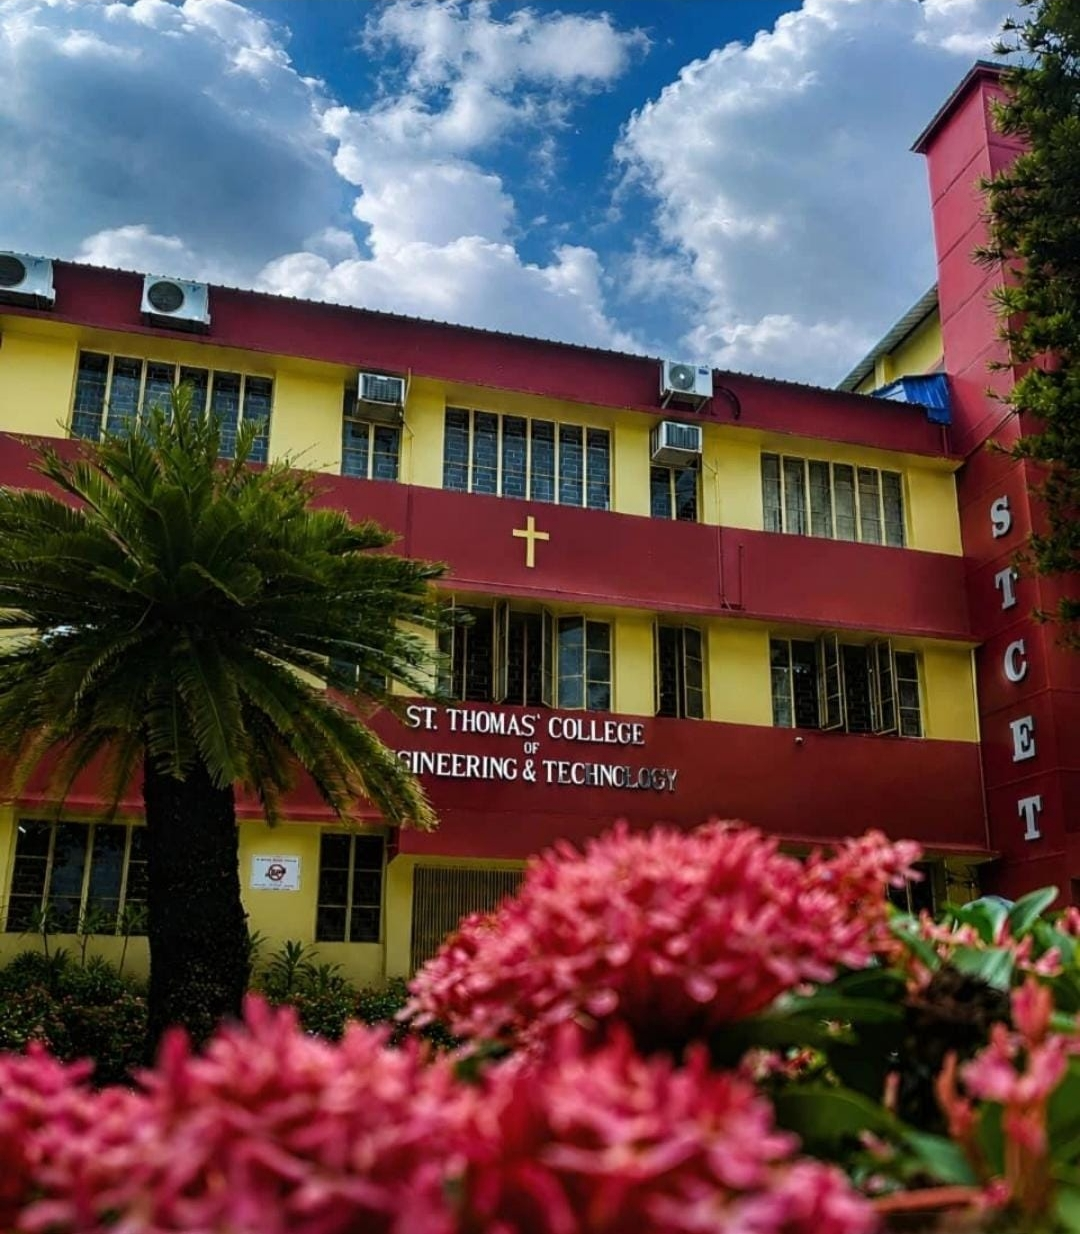
\includegraphics[width=0.5\textwidth, height=8cm]{assets/images/college-pic-3.jpeg}%
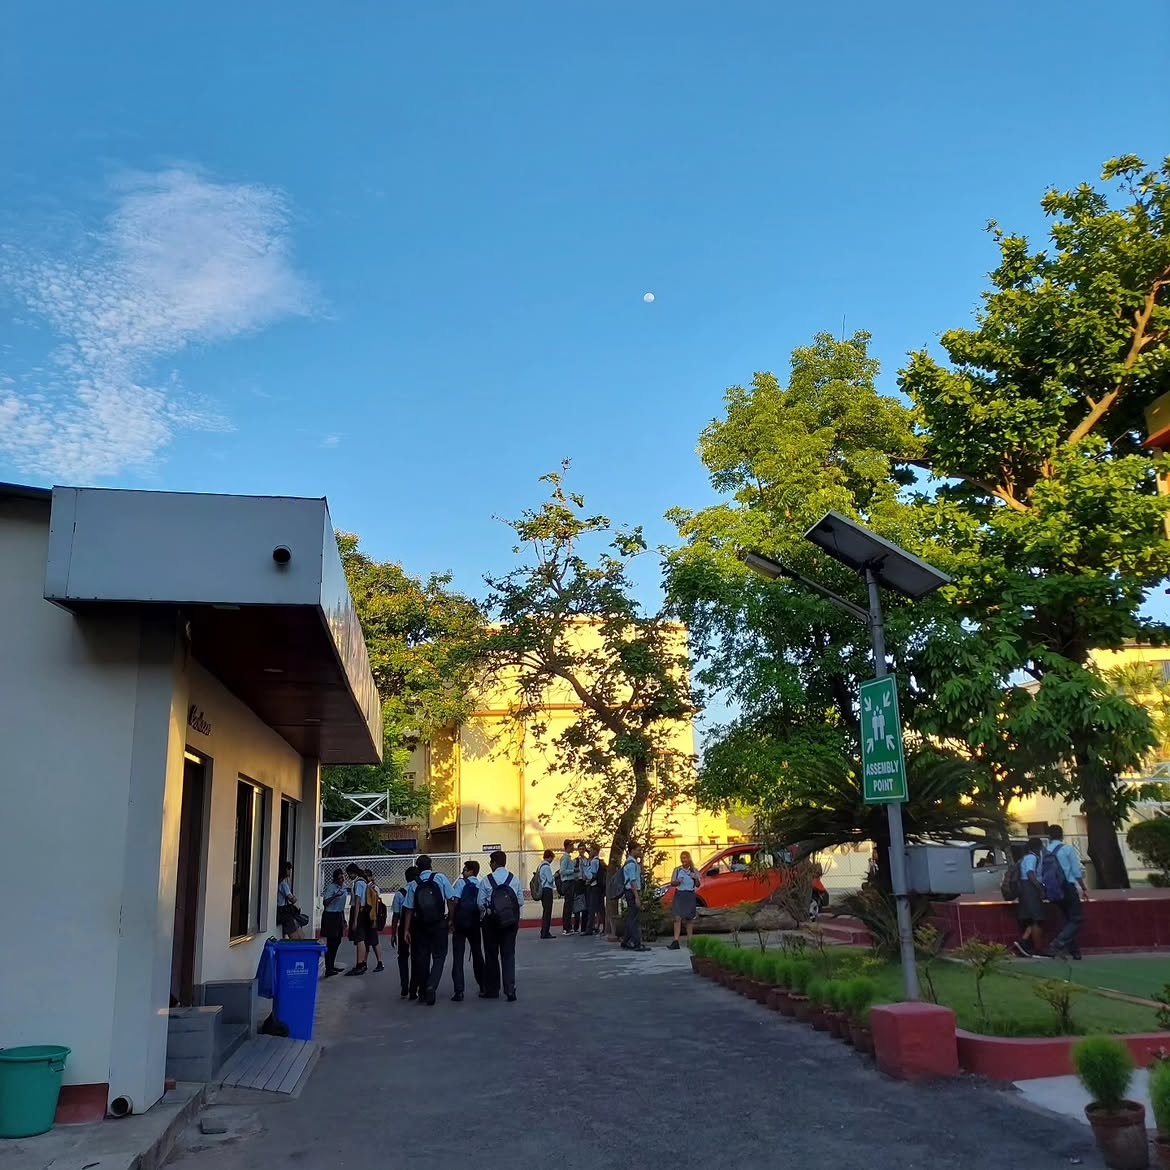
\includegraphics[width=0.5\textwidth, height=8cm]{assets/images/college-pic-2.jpeg}
\newpage
\begin{center}
  \section*{Vision of \\Electronics \& Communication Engineering Department}
\end{center}

\justify
To foster excellence in teaching and research to converge multidisciplinary approach, and sustainability with ethical values for evolving industrial and academic needs in Electronics and Communication Engineering.

\begin{center}
  \section*{Mission of \\Electronics \& Communication Engineering Department}
\end{center}

\begin{itemize}
  \item \textbf{M1:} To produce industry-ready Electronics and Communication professionals through innovative, lab-based and project-driven education in a modern environment.
  \item \textbf{M2:} To advance research in Electronics and Communication Engineering for the competitive and sustainable development of the country.
  \item \textbf{M3:} To develop the department as a learning center for advancing Electronics and Communication Engineering with social values, environmental awareness and entrepreneurial mindset.
\end{itemize}

\noindent
\begin{minipage}[t]{0.5\textwidth}
  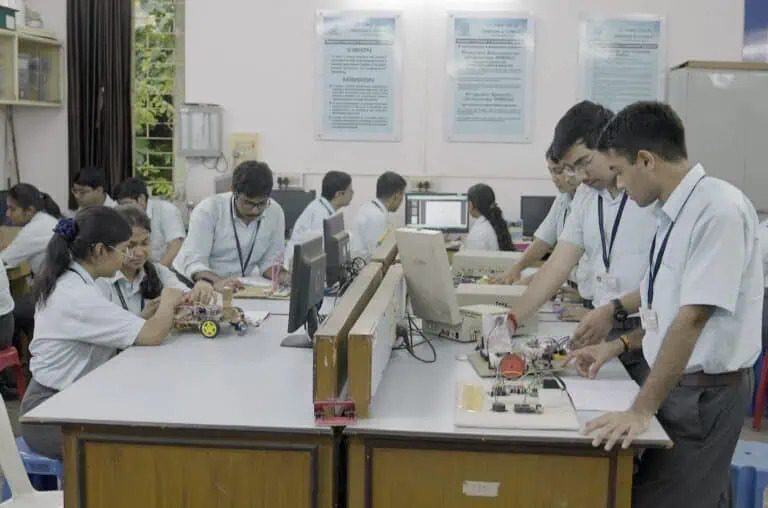
\includegraphics[width=\linewidth, height=6cm]{assets/images/ece-1.jpg}
\end{minipage}%
\begin{minipage}[t]{0.5\textwidth}
  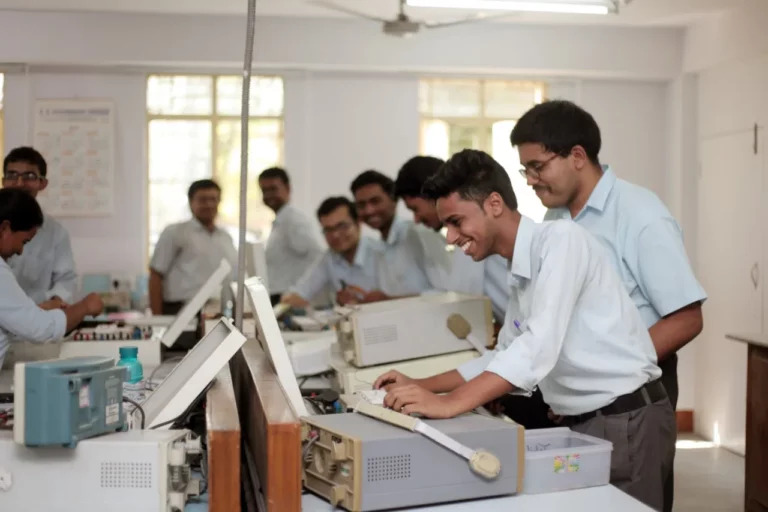
\includegraphics[width=\linewidth, height=6cm]{assets/images/ece-3.jpg}
\end{minipage}

\newpage
\begin{center}
  \section*{Program Educational Objectives (PEOs)}
\end{center}
\justify
Graduates of the Electronics and Communication Engineering program shall:
\begin{itemize}
  \item \textbf{PEO1:} Possess design skills and core proficiency in Electronics \& Communication Engineering for employment in relevant industries.
  \item \textbf{PEO2:} Possess strong core and advanced knowledge in Electronics \& Communication Engineering to pursue higher studies.
  \item \textbf{PEO3:} Exhibit leadership, ethical values, and social commitment to contribute in academia, industry and/or entrepreneurial ventures, both nationally and globally.
\end{itemize}

\begin{center}
  \section*{Program Specific Outcomes (PSOs)}
\end{center}
\justify
After completion of the program, a graduate engineer would have an ability to:
\begin{itemize}
  \item \textbf{PSO1. Professional skills:} Solve real life problems relevant to Electronics and Communication Engineering in various areas, like VLSI, Nano-technology, Advanced Communications, Signal Processing, Embedded Systems, IoT and applications involving AI \& ML.
  \item \textbf{PSO2. Competency:} Demonstrate competence in qualifying exams and pursue successful careers in employment, research and higher education at state, national, and international levels.
\end{itemize}

\begin{figure}[h]
  \centering
  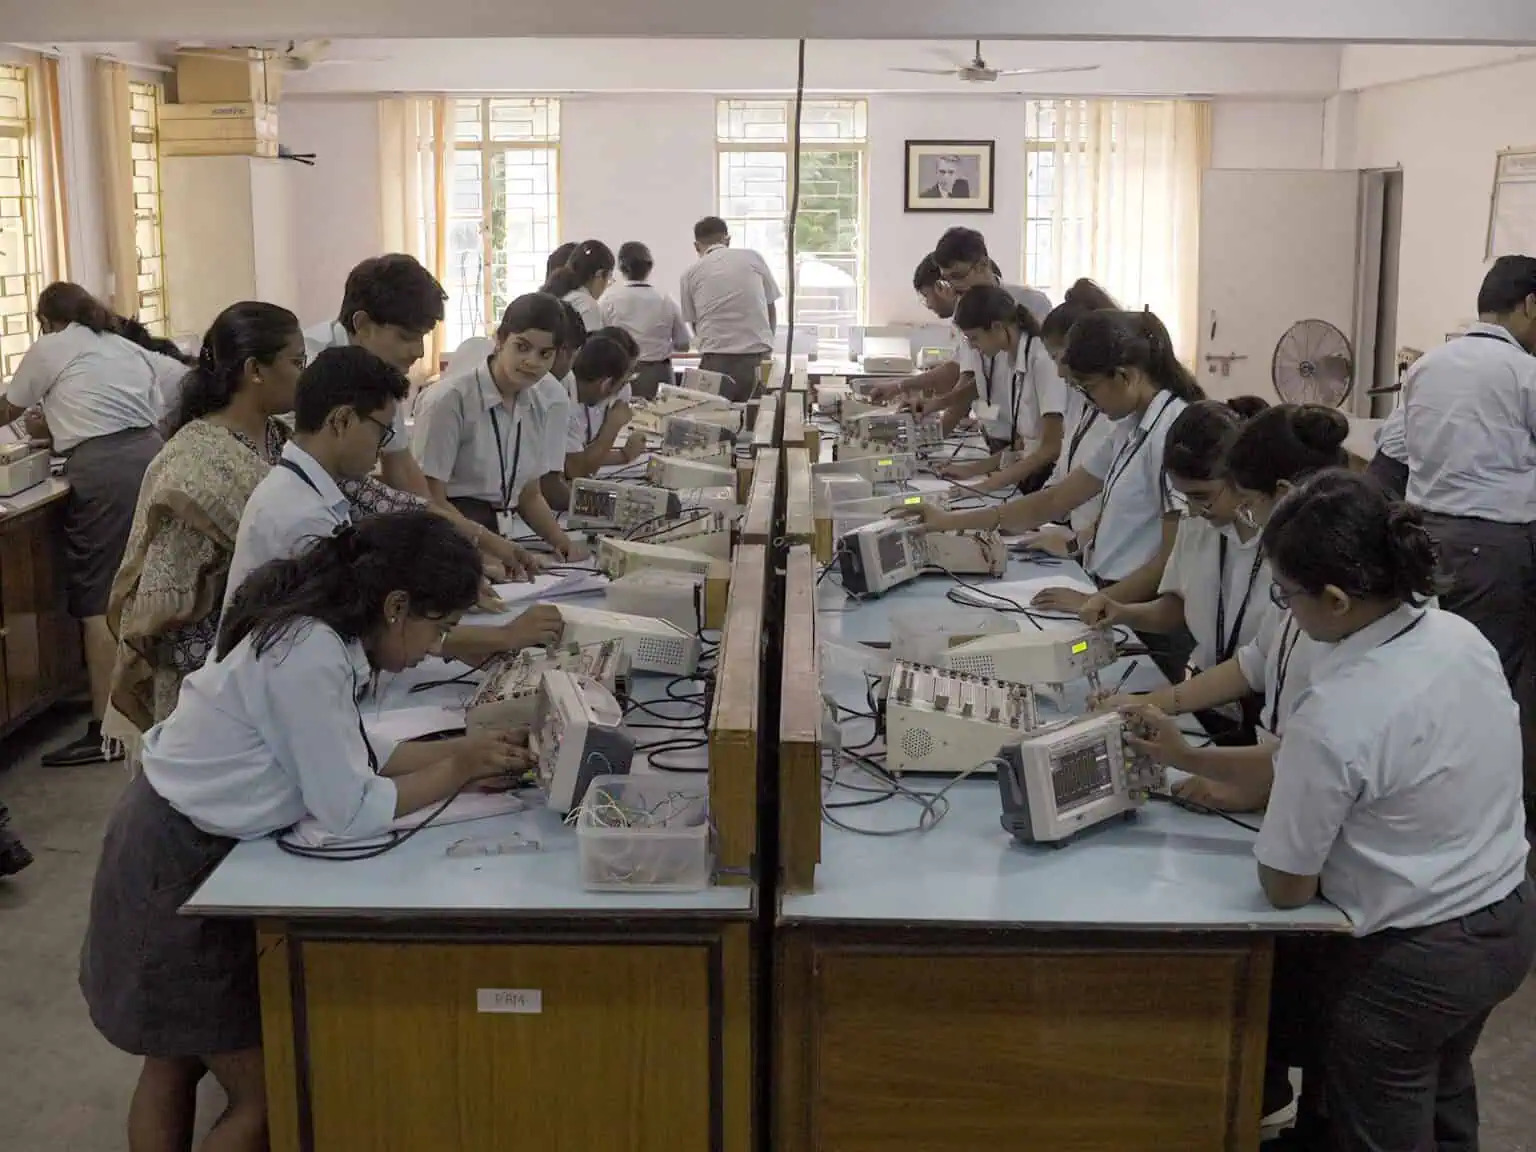
\includegraphics[width=\textwidth, keepaspectratio]{assets/images/ece-2.jpg}
\end{figure}

\newpage

\begin{center}
  \section*{About the Department of Electronics \& Communication Engineering}
\end{center}

\justify
The Department of Electronics and Communication Engineering (ECE) at St. Thomas College of Engineering \& Technology represents the pinnacle of technical education, delivering a comprehensive curriculum that seamlessly integrates core electronics principles with emerging technologies. Our program emphasizes mastery of analog and digital circuit design, electromagnetic theory, communication systems, and microprocessor architecture, preparing students for the full spectrum of ECE career paths.

\vspace{0.5em}

State-of-the-art laboratories equipped with cutting-edge instrumentation—including network analyzers, logic analyzers, high-frequency oscilloscopes, and advanced PCB design workstations—enable practical implementation of complex systems. Specialized facilities support research in RF/microwave engineering, embedded systems development, VLSI prototyping, and digital signal processing applications critical to modern telecommunications infrastructure.

\vspace{0.5em}

\justify
Faculty expertise spans semiconductor device physics, antenna design, wireless protocol development, and machine learning applications in signal processing, supported by ongoing research funded through national grants and industry partnerships. Our graduates excel in core technical roles across semiconductor fabrication, telecommunications infrastructure, embedded systems design, and defense electronics, consistently securing positions with leading organizations in India's rapidly expanding electronics sector.

\begin{figure}[h]
  \centering
  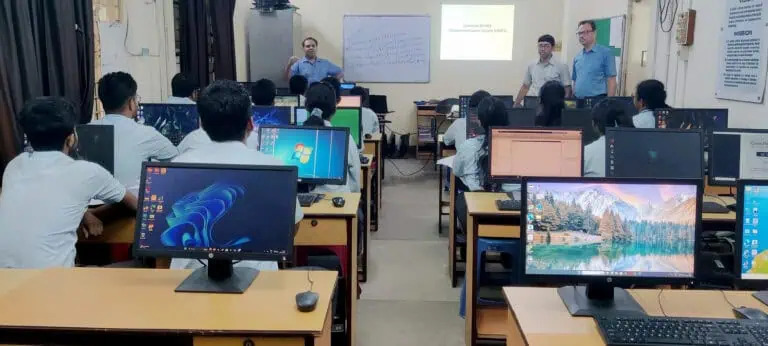
\includegraphics[width=\textwidth, keepaspectratio]{assets/images/ece-4.jpg}
\end{figure}